\documentclass[11pt]{article}

\usepackage[margin=1in]{geometry}
\usepackage{microtype}
\usepackage{setspace}
\setstretch{1.03}

\usepackage{amsmath,amssymb}
\usepackage{array}
\usepackage{booktabs}
\usepackage{siunitx}
\usepackage{graphicx}
\usepackage{float}
\usepackage{caption}
\usepackage{longtable}
\usepackage{tabularx}
\usepackage{tikz}
\usepackage{mdframed}
\usepackage{xcolor}
\usepackage{fancyhdr}
\usepackage{hyperref}
\usepackage[nameinlink,capitalize]{cleveref}
\usetikzlibrary{arrows.meta}

\graphicspath{{figures/}}
\hypersetup{
  colorlinks=true,
  linkcolor=blue!50!black,
  urlcolor=blue!50!black,
  citecolor=blue!50!black,
  pdftitle={Childcare Desert Reduction in New York City},
  pdfauthor={Group 8}
}
\sisetup{group-separator={,},group-minimum-digits=4}
\renewcommand{\refname}{Bibliography}
\newcolumntype{L}[1]{>{\raggedright\arraybackslash}p{#1}}
\newcolumntype{Y}{>{\raggedright\arraybackslash}X}

\newcommand{\coursecode}{IEOR E4004}
\newcommand{\coursetitle}{Optimization Models and Methods}
\newcommand{\assignmenttitle}{Project I --- Childcare Desert Reduction in New York City}
\newcommand{\term}{Spring~2026}
\newcommand{\instructor}{Prof.\ Dr. Yaren Bilge Kaya}
\newcommand{\studentname}{Group 8}
\newcommand{\dueday}{March 2026}
\newcommand{\logoimg}{ieor.png}

\newmdenv[
  linewidth=0.5pt,
  roundcorner=4pt,
  backgroundcolor=black!2,
  skipabove=\baselineskip,
  skipbelow=\baselineskip,
  innertopmargin=6pt,
  innerbottommargin=6pt,
  innerleftmargin=9pt,
  innerrightmargin=9pt
]{resultbox}

\fancypagestyle{coverstyle}{%
  \fancyhf{}
  \lhead{Columbia University}
  \chead{\coursecode}
  \rhead{\studentname}
  \cfoot{\thepage}
  \renewcommand{\headrulewidth}{0.5pt}
  \renewcommand{\footrulewidth}{0.5pt}
}
\pagestyle{fancy}
\fancyhf{}
\lhead{\coursecode}
\rhead{\assignmenttitle}
\cfoot{\thepage}
\setlength{\headheight}{14pt}
\renewcommand{\headrulewidth}{0.5pt}
\renewcommand{\footrulewidth}{0.5pt}

\begin{document}
\hypersetup{pageanchor=false}
\pagenumbering{Roman}

% --- Title page ---
\begin{titlepage}
  \thispagestyle{coverstyle}
  \centering
  \vspace*{0.2cm}
  \if\relax\detokenize{\logoimg}\relax\else
    \includegraphics[width=0.34\textwidth]{\logoimg}
  \fi

  \vspace{0.5cm}
  {\Large \textsc{\coursecode{} --- \coursetitle{}} \par}
  \vspace{0.2cm}
  {\LARGE \textbf{\assignmenttitle} \par}
  \vspace{0.3cm}
  {\large \term \par}
  \vspace{0.6cm}
  \noindent\makebox[\linewidth]{\rule{\linewidth}{1.2pt}}

  \vspace{0.9cm}
  \begin{minipage}{0.48\textwidth}
    \raggedright
    \textit{Team}\\
    Alexandre Sep\'ulveda de Dietrich (aes2399)\\
    Rong Ji (rj2754)\\
    Suyi Li (sl5867)\\
    Zichen He (zh2709)\\
    Zipeng Liu (zl3627)
  \end{minipage}\hfill
  \begin{minipage}{0.48\textwidth}
    \raggedleft
    \textit{Instructor}\\
    \instructor\\[4pt]
    \textit{Due}\\
    \dueday
  \end{minipage}

  \vfill
  {\large Department of Industrial Engineering and Operations Research\\Columbia University}
\end{titlepage}

\setcounter{page}{2}
\tableofcontents
\newpage
\hypersetup{pageanchor=true}
\pagenumbering{arabic}

This project studies how New York City can reduce childcare deserts at minimum cost by combining expansions of existing childcare facilities with the opening of new facilities.
New York City classifies a zip code as a childcare desert when licensed capacity is too low relative to local child population. 

In high-demand areas, defined as zip codes with employment rate at least \(60\%\) or average income at most \(\$60{,}000\), the relevant threshold is one half of the population aged \(0\) to \(12\); otherwise it is one third. NYC also imposes a separate requirement for children aged \(0\) to \(5\): available under-\(5\) slots should be at least two thirds of the local \(0\) to \(5\) population \cite{assignment}.

This project studies the minimum public funding needed to eliminate coded childcare deserts across NYC. We solve the problem in two stages: Part 1 builds an implemented benchmark model that allows free siting of new facilities and more flexible expansion of existing ones. Part 2 keeps the same demand logic but imposes tighter expansion caps, candidate-site restrictions, and spacing rules, producing a more operational planning model.

\paragraph{Code availability.}
The working code is organized as a seven-stage notebook pipeline in the submitted repository: shared data cleaning, benchmark parameter estimation, benchmark optimization, benchmark visualization, realistic parameter estimation, realistic optimization and validation, and final comparison visualization. The workflow first constructs shared inputs, then solves Part 1, then solves Part 2, and finally exports the tables and figures used in this report. The submitted repository is available at \url{https://github.com/alexandre-sdd/childcare_deserts_nyc}; it contains the notebook pipeline under \texttt{notebooks/} and the report files under \texttt{report/}. \Cref{fig:code-pipeline-aligned} gives a compact schema of that pipeline.

\begin{figure}[H]
\centering
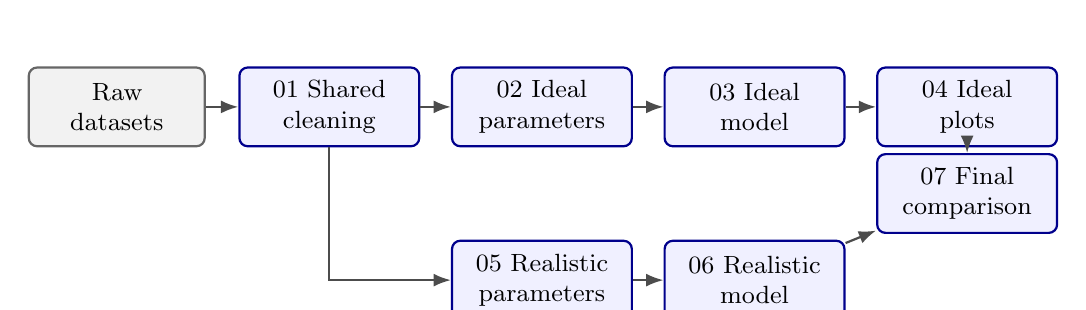
\begin{tikzpicture}[
  font=\small,
  stage/.style={
    draw=blue!55!black,
    thick,
    rounded corners=3pt,
    fill=blue!6,
    align=center,
    minimum height=1.0cm,
    text width=2.05cm
  },
  source/.style={
    draw=black!60,
    thick,
    rounded corners=3pt,
    fill=black!5,
    align=center,
    minimum height=1.0cm,
    text width=2.0cm
  },
  flow/.style={-{Latex[length=2.2mm]}, thick, draw=black!70}
]
  \node[source] (raw) at (0,0) {Raw\\datasets};
  \node[stage] (s1) at (2.7,0) {01 Shared\\cleaning};
  \node[stage] (s2) at (5.4,0) {02 Ideal\\parameters};
  \node[stage] (s3) at (8.1,0) {03 Ideal\\model};
  \node[stage] (s4) at (10.8,0) {04 Ideal\\plots};
  \node[stage] (s5) at (5.4,-2.2) {05 Realistic\\parameters};
  \node[stage] (s6) at (8.1,-2.2) {06 Realistic\\model};
  \node[stage] (s7) at (10.8,-1.1) {07 Final\\comparison};

  \draw[flow] (raw) -- (s1);
  \draw[flow] (s1) -- (s2);
  \draw[flow] (s2) -- (s3);
  \draw[flow] (s3) -- (s4);
  \draw[flow] (s1) |- (s5);
  \draw[flow] (s5) -- (s6);
  \draw[flow] (s4) -- (s7);
  \draw[flow] (s6) -- (s7);
\end{tikzpicture}
\caption{Notebook pipeline used to construct shared inputs, solve both models, and export report figures.}
\label{fig:code-pipeline-aligned}
\end{figure}

\section{Background and Problem Framing}

Childcare deserts matter because lack of access affects both labor-force participation and early-childhood care, a point emphasized in the broader childcare-desert literature summarized by the Center for American Progress \cite{americanprogress}. The project framing here is operational rather than behavioral: demand is enforced at the zip-code level, and the government decides how much to spend on two levers, expanding existing facilities and opening new ones. That makes the problem well suited to mixed-integer optimization, but it also means the results should be interpreted as planning solutions rather than household travel models.

\section{Parameter Estimation}

\subsection{Shared data cleaning}

The notebook pipeline uses five raw datasets supplied with the assignment: regulated childcare facilities, potential locations, employment rates, average individual income, and child population by zip code. The shared-cleaning stage standardizes zip codes, harmonizes columns, converts numeric fields, and preserves facilities even when geographic coordinates are missing.

\Cref{tab:shared-clean-structure} shows the cleaned shared tables passed from Notebook 01 to the later parameter-estimation and optimization stages.

\begin{table}[H]
\centering
\footnotesize
\renewcommand{\arraystretch}{1.08}
\begin{tabularx}{\textwidth}{L{3.8cm}L{1.6cm}Y}
\toprule
\textbf{Shared output} & \textbf{Level} & \textbf{Used for} \\
\midrule
Clean facility table & facility & Standardized facility master table with active flag, geo flag, under-\(5\) proxy, and quality flags \\
Facility geo-ready table & facility & Compact facility subset used for realistic distance screening \\
Clean population table & zipcode & Harmonized age bands plus derived child-population fields \\
Clean employment table & zipcode & Zipcode employment covariate before imputation \\
Clean income table & zipcode & Zipcode income covariate before imputation \\
Candidate geo-ready table & candidate & Standardized candidate ID, zip code, coordinates, and geo flag \\
Master zipcode universe & zipcode & Merge backbone with source flags, facility counts, baseline capacity, and candidate counts \\
\bottomrule
\end{tabularx}
\caption{Shared cleaned outputs generated by Notebook 01}
\label{tab:shared-clean-structure}
\end{table}

Three modeling choices in the shared pipeline materially affect later steps. First, active facilities with positive licensed capacity define the incumbent supply universe. Second, \texttt{children\_capacity} is used as the under-\(5\) capacity proxy for existing facilities. Third, missing employment and income values are imputed with citywide medians, while missing child-population entries are carried as zero after the merged zip-code table is formed. The processed ideal inputs cover \(311\) zip codes and \(7{,}712\) active facilities.

\subsection{Demand- and supply-side parameters}

For each zip code \(z\), the benchmark stage defines the high-demand indicator as
\[
\text{high\_demand}_z =
\mathbf{1}\{\text{employment}_z \ge 0.60 \ \text{or}\ \text{income}_z \le 60{,}000\}.
\]
The corresponding total-capacity requirement is
\[
\mathrm{req\_total}_z =
\begin{cases}
\left\lfloor 0.5 \cdot \mathrm{pop}_{0\text{--}12,z} \right\rfloor + 1, & \text{high demand},\\[0.5ex]
\left\lfloor \frac{1}{3} \cdot \mathrm{pop}_{0\text{--}12,z} \right\rfloor + 1, & \text{otherwise},
\end{cases}
\]
and the under-\(5\) requirement is
\[
\mathrm{req\_under5}_z = \left\lceil \frac{2}{3}\,\mathrm{pop}_{0\text{--}5,z} \right\rceil.
\]
When observed child population is zero, the implemented pipeline sets \(\mathrm{req\_total}_z=0\) and does not classify the zip code as a baseline total-capacity desert. Existing supply is aggregated from facility-level licensed capacity and under-\(5\) proxy capacity within each zip code.

\subsection{Intervention parameters}

New-facility options are unchanged across both parts and come directly from the assignment.

\begin{table}[H]
\centering
\small
\begin{tabular}{lrrr}
\toprule
\textbf{Facility type} & \textbf{Total slots} & \textbf{Under-\(5\) max} & \textbf{Fixed cost (\$)} \\
\midrule
Small & 100 & 50 & 65,000 \\
Medium & 200 & 100 & 95,000 \\
Large & 400 & 200 & 115,000 \\
\bottomrule
\end{tabular}
\caption{New-facility build menu used in both models}
\label{tab:build-menu}
\end{table}

\paragraph{Part 1 benchmark parameters.}
For both parts, \(n_f\) denotes the current licensed capacity at facility \(f\). In Part 1, \(x_f\) denotes the total added slots at that facility. The instructor-approved expansion-cap interpretation used in the notebook is
\[
x_f \le \min(1.2 n_f,\ 500).
\]
Because the assignment does not specify the first-block cost function \(c_{\text{slots}}(n_f)\), the benchmark parameter-estimation stage uses
\[
c_f^{(1)} =
\begin{cases}
350, & n_f < 25,\\
300, & 25 \le n_f < 75,\\
250, & n_f \ge 75,
\end{cases}
\qquad \text{dollars per added slot,}
\]
and, for expansions at or above current capacity,
\[
c_f^{(2)} = \frac{20000 + 200\,n_f}{n_f}.
\]
The implemented Part 1 model then prices each facility's expansion at \(c_f^{(1)}\) if \(x_f < n_f\) and at \(c_f^{(2)}\) if \(x_f \ge n_f\).

\paragraph{Part 2 realistic parameters.}
The realistic parameter-estimation stage no longer treats expansion as one undifferentiated total. Instead, it partitions the allowed increase at each facility into three incremental integer bands: the first \(10\%\) of current capacity, the next \(5\%\), and the final \(5\%\), with an overall \(20\%\) cap. The floor operators convert those percentage thresholds into slot counts while keeping the total limit equal to \(\lfloor 0.20\,n_f \rfloor\):
\[
\mathrm{cap1}_f = \left\lfloor 0.10\,n_f \right\rfloor,\qquad
\mathrm{cap2}_f = \left\lfloor 0.15\,n_f \right\rfloor - \left\lfloor 0.10\,n_f \right\rfloor,\qquad
\mathrm{cap3}_f = \left\lfloor 0.20\,n_f \right\rfloor - \left\lfloor 0.15\,n_f \right\rfloor.
\]
So \(\mathrm{cap1}_f\) is the size of the first band, \(\mathrm{cap2}_f\) is the additional room between \(10\%\) and \(15\%\), and \(\mathrm{cap3}_f\) is the additional room between \(15\%\) and \(20\%\). The associated block-cost coefficients are
\[
\mathrm{coef1}_f = \frac{20000 + 200\,n_f}{n_f},\qquad
\mathrm{coef2}_f = \frac{20000 + 400\,n_f}{n_f},\qquad
\mathrm{coef3}_f = \frac{20000 + 1000\,n_f}{n_f}.
\]
Later, the optimization model uses decision variables \(x_{1f},x_{2f},x_{3f}\) for those three bands, so total added slots are \(x_f := x_{1f}+x_{2f}+x_{3f}\). Under the original assignment Part 2 rule, the total expansion cost is
\[
C_f(x_f)=
\begin{cases}
\mathrm{coef1}_f x_f, & 0 \le x_f \le \left\lfloor 0.10\,n_f \right\rfloor,\\
\mathrm{coef2}_f x_f, & \left\lfloor 0.10\,n_f \right\rfloor < x_f \le \left\lfloor 0.15\,n_f \right\rfloor,\\
\mathrm{coef3}_f x_f, & \left\lfloor 0.15\,n_f \right\rfloor < x_f \le \left\lfloor 0.20\,n_f \right\rfloor.
\end{cases}
\]
This discontinuous regime-based total-cost rule creates upward jumps at the \(10\%\) and \(15\%\) thresholds because the higher regime coefficient applies to the full expansion level, not just to the incremental block. The processed inputs imply a citywide realistic expansion room of \(61{,}197\) slots. \Cref{fig:realistic-expansion-functions} illustrates the assignment-style example \(n_f=100\), where the breakpoints occur at \(10\), \(15\), and \(20\) added slots. In the implemented optimization model, these same coefficients are used in an additive increasing-cost objective for tractability.

\begin{figure}[H]
\centering
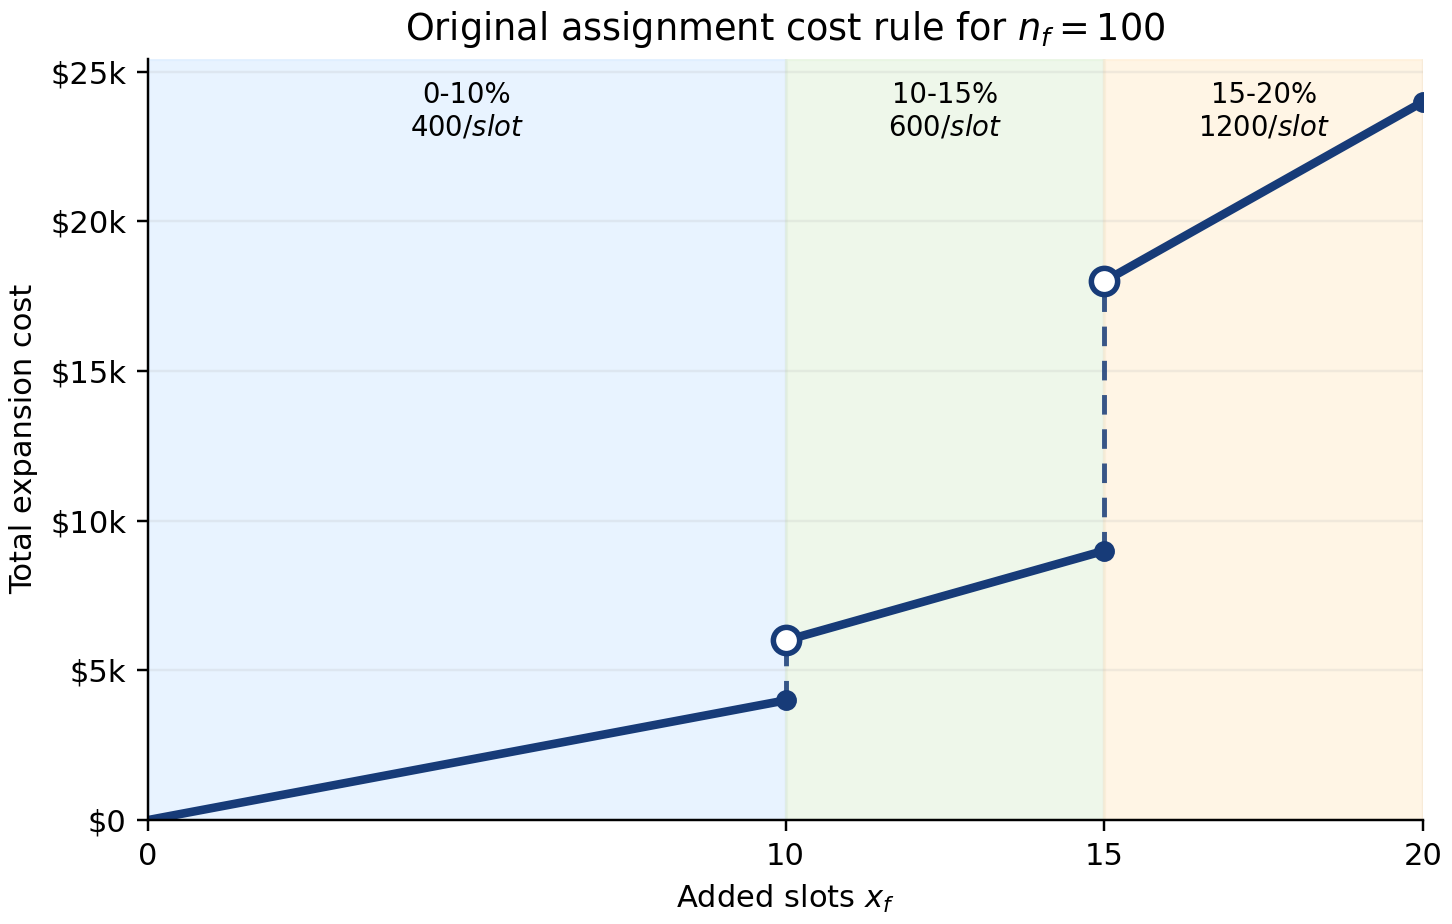
\includegraphics[width=0.8\textwidth]{realistic_expansion_functions.png}
\caption{Total realistic expansion cost rule for the example \(n_f=100\). Dashed vertical segments mark the jumps at the \(10\%\) and \(15\%\) thresholds, where the higher regime coefficient applies to the entire expansion amount.}
\label{fig:realistic-expansion-functions}
\end{figure}

\begin{table}[H]
\centering
\small
\renewcommand{\arraystretch}{1.05}
\begin{tabularx}{0.86\textwidth}{L{2.7cm}Y r}
\toprule
\textbf{Block} & \textbf{Metric} & \textbf{Value} \\
\midrule
\multicolumn{3}{l}{\textit{Candidate screening}} \\
Sites & Candidate sites examined & 31,100 \\
Sites & Blocked candidate sites & 2,578 \\
Sites & Feasible candidate sites & 28,522 \\
\addlinespace[2pt]
\multicolumn{3}{l}{\textit{Conflict structure}} \\
Pairs & Candidate-candidate conflict pairs & 11,455 \\
Pairs & Candidate-existing conflict pairs & 4,730 \\
Pairs & Existing-existing close pairs (diagnostic only) & 7,644 \\
\addlinespace[2pt]
\multicolumn{3}{l}{\textit{Data quality}} \\
Missing geo & Facilities missing coordinates & 169 \\
\bottomrule
\end{tabularx}
\caption{Part 2 site-screening outputs from the realistic parameter-estimation stage}
\label{tab:screening}
\end{table}

\section{Methods}

\subsection{Part 1 benchmark model}

The benchmark model is defined over zip codes \(z \in Z\), active existing facilities \(f \in F\), and build sizes \(s \in S=\{\text{small},\text{medium},\text{large}\}\). For zipcode-level aggregation, \(F(z)\) denotes the set of existing facilities in zipcode \(z\). The key decision variables are
\[
\begin{aligned}
x_f &= \text{total expansion slots at facility } f,\\
u_f &= \text{under-\(5\) slots assigned within expansion},\\
\delta_f &= \text{binary indicator for the high-cost expansion regime},\\
w_f &= \text{auxiliary facility expansion-cost variable},\\
y_{zs} &= \text{number of new facilities of size } s \text{ in zip } z,\\
g_{zs} &= \text{under-\(5\) slots assigned within those new builds}.
\end{aligned}
\]

The objective is to minimize modeled expansion cost, fixed build cost, and \(\$100\) for each newly created under-\(5\) slot:
\[
\min \sum_{f \in F} w_f
 + \sum_{z \in Z}\sum_{s \in S} K_s y_{zs}
 + 100\left(\sum_{f \in F}u_f+\sum_{z \in Z}\sum_{s \in S}g_{zs}\right).
\]
The core constraints enforce facility-level expansion caps, under-\(5\) assignment limits, threshold logic for the two cost regimes, and zip-code service requirements:

\noindent\textit{Facility-level cap and regime constraints.}
\[
\begin{alignedat}{2}
x_f &\le U_f, &\qquad u_f &\le x_f,\\
x_f &\le (n_f-1)+U_f\delta_f, &\qquad x_f &\ge n_f\delta_f,
\end{alignedat}
\]

\noindent\textit{Cost-linking constraints.}
\[
\begin{aligned}
w_f &\ge c_f^{(1)}x_f - M_f^{\mathrm{cost}}\delta_f,\\
w_f &\le c_f^{(1)}x_f + M_f^{\mathrm{cost}}\delta_f,\\
w_f &\ge c_f^{(2)}x_f - M_f^{\mathrm{cost}}(1-\delta_f),\\
w_f &\le c_f^{(2)}x_f + M_f^{\mathrm{cost}}(1-\delta_f).
\end{aligned}
\]
Here \(M_f^{\mathrm{cost}}\) is a sufficiently large constant that activates the appropriate regime, so the full expansion at facility \(f\) is priced under either \(c_f^{(1)}\) or \(c_f^{(2)}\).

\noindent\textit{Zipcode service constraints and under-\(5\) build limits.}
\[
\begin{aligned}
\mathrm{existing\_total}_z + \sum_{f \in F(z)}x_f + \sum_{s \in S}B_s y_{zs}
&\ge \mathrm{req\_total}_z,\\
\mathrm{existing\_under5}_z + \sum_{f \in F(z)}u_f + \sum_{s \in S}g_{zs}
&\ge \mathrm{req\_under5}_z,\\
g_{zs} &\le U_s y_{zs}.
\end{aligned}
\] The implemented model also includes non-negativity and integrality constraints on the decision variables, but those are omitted here for clarity.

This model is intentionally optimistic. It does not represent siting feasibility, minimum spacing, or cross-zip travel. It is best interpreted as the implemented benchmark model rather than a deployable plan.

\begin{resultbox}
\textbf{Implemented Part 1 model.}
The benchmark optimization stage solves a citywide MILP with \(32{,}714\) variables and \(63{,}251\) constraints. The model enforces zipcode-level total and under-\(5\) service targets through facility expansion and zipcode-level new-build decisions, but it does not impose candidate-site or spacing restrictions.
\end{resultbox}

\subsection{Part 2 realistic model}

The realistic model keeps the same demand targets but changes the intervention structure. Existing facilities may expand only within three capped bands, and new facilities can only be opened on observed candidate sites \(l \in L\). For zipcode-level aggregation, \(L(z)\) denotes the set of candidate sites in zipcode \(z\). The key parameters are the three incumbent expansion caps \(\mathrm{cap1}_f,\mathrm{cap2}_f,\mathrm{cap3}_f\), the corresponding coefficients \(\mathrm{coef1}_f,\mathrm{coef2}_f,\mathrm{coef3}_f\), the blocked-site set \(L_{\text{blocked}}\), the within-zipcode conflict set \(\mathcal{C}\), and the build-menu parameters \(K_s,B_s,U_s\). The key decision variables are
\[
\begin{aligned}
x_{1f},x_{2f},x_{3f} &= \text{added slots in the }0\%\text{--}10\%,\,10\%\text{--}15\%,\,15\%\text{--}20\%\text{ bands},\\
u_f &= \text{under-\(5\) slots assigned within incumbent expansion},\\
y_{ls} &= \text{binary indicator for opening size } s \text{ at candidate site } l,\\
g_{ls} &= \text{under-\(5\) slots assigned within that selected facility.}
\end{aligned}
\]

The implemented objective is
\[
\min \sum_{f \in F}\left(\mathrm{coef1}_f x_{1f}+\mathrm{coef2}_f x_{2f}+\mathrm{coef3}_f x_{3f}\right)
 + \sum_{l \in L}\sum_{s \in S} K_s y_{ls}
 + 100\left(\sum_{f \in F}u_f+\sum_{l \in L}\sum_{s \in S}g_{ls}\right).
\]
The main feasibility constraints are

\noindent\textit{Incumbent expansion-band constraints.}
\[
\begin{aligned}
x_{1f} \le \mathrm{cap1}_f,\qquad
x_{2f} \le \mathrm{cap2}_f,\qquad
x_{3f} \le \mathrm{cap3}_f
&\qquad \forall f \in F,\\
u_f \le x_{1f}+x_{2f}+x_{3f}
&\qquad \forall f \in F.
\end{aligned}
\]

\noindent\textit{Candidate-site selection, under-\(5\) assignment, and implemented spacing constraints.}
\[
\begin{aligned}
\sum_{s \in S} y_{ls} &\le 1 && \forall l \in L,\\
g_{ls} &\le U_s y_{ls} && \forall l \in L,\ \forall s \in S,\\
\sum_{s \in S} y_{ls} &= 0 && \forall l \in L_{\text{blocked}},\\
\sum_{s \in S} y_{l_1s} + \sum_{s \in S} y_{l_2s}
&\le 1 && \forall (l_1,l_2)\in \mathcal{C}.
\end{aligned}
\]

\noindent\textit{Zipcode service constraints.}
\[
\begin{aligned}
\mathrm{existing\_total}_z + \sum_{f \in F(z)}(x_{1f}+x_{2f}+x_{3f}) + \sum_{l \in L(z)}\sum_{s \in S} B_s y_{ls}
&\ge \mathrm{req\_total}_z && \forall z \in Z,\\
\mathrm{existing\_under5}_z + \sum_{f \in F(z)}u_f + \sum_{l \in L(z)}\sum_{s \in S} g_{ls}
&\ge \mathrm{req\_under5}_z && \forall z \in Z.
\end{aligned}
\]
These choices preserve the intended planning logic while keeping the implemented model tractable. Banded incumbent variables make the tighter \(20\%\) cap and increasing marginal expansion difficulty transparent, while candidate-site binary variables enforce the coded \(0.06\)-mile screening rules used for candidate-site selection. Because existing facilities are fixed assets in the current planning horizon, existing-existing proximity issues are tracked as diagnostics rather than modeled as closures or relocations.

\begin{resultbox}
\textbf{Implemented Part 2 model.}
The realistic optimization stage solves a citywide MILP with \(201{,}980\) variables and \(155{,}819\) constraints. The model enforces zipcode service constraints together with the implemented candidate-site screening rules, but the expansion-cost objective is an additive increasing-cost approximation rather than the assignment's literal piecewise-total formula. Existing-existing distance conflicts are recorded diagnostically, not enforced.
\end{resultbox}

\section{Results}

\subsection{Part 1 benchmark results}

The implemented benchmark objective is \(\$126.67\) million.

\begin{resultbox}
\textbf{Benchmark takeaway.}
The implemented benchmark requires \(\$126.67\) million, including \(206{,}364\) expansion slots, \(386\) new facilities, and \(135\) facilities that cross into the higher-cost expansion regime. Even under optimistic siting assumptions, new construction is still necessary.
\end{resultbox}

\begin{table}[H]
\centering
\small
\renewcommand{\arraystretch}{1.05}
\begin{tabularx}{0.92\textwidth}{L{2.4cm}Y r}
\toprule
\textbf{Block} & \textbf{Metric} & \textbf{Value} \\
\midrule
\multicolumn{3}{l}{\textit{Costs}} \\
Objective & Total objective (\$) & 126,668,941 \\
Objective & Expansion cost (\$) & 54,716,841 \\
Objective & New-build cost (\$) & 44,180,000 \\
Objective & Under-\(5\) equipment cost (\$) & 27,772,100 \\
\addlinespace[2pt]
\multicolumn{3}{l}{\textit{Capacity added}} \\
Expansion & Added expansion slots & 206,364 \\
Expansion & Added under-\(5\) expansion slots & 202,938 \\
New build & Added new-build slots & 152,900 \\
New build & Added under-\(5\) new-build slots & 74,783 \\
\addlinespace[2pt]
\multicolumn{3}{l}{\textit{Facilities and coverage}} \\
Facilities & New facilities built & 386 \\
Coverage & Zip codes meeting all coded requirements after solve & 311 \\
\bottomrule
\end{tabularx}
\caption{Implemented Part 1 benchmark results}
\label{tab:part1-results}
\end{table}

\subsection{Part 2 realistic results}

The implemented realistic objective is \(\$183.96\) million.

\begin{resultbox}
\textbf{Realistic-model takeaway.}
The implemented realistic model costs \(\$183.96\) million. Expansion falls to \(25{,}108\) slots, while new construction rises to \(1{,}284\) facilities and \(507{,}700\) new slots.
\end{resultbox}

\begingroup
\small
\renewcommand{\arraystretch}{1.05}
\begin{longtable}{L{2.4cm}L{8.0cm}r}
\caption{Implemented Part 2 realistic results}\label{tab:part2-results}\\
\toprule
\textbf{Block} & \textbf{Metric} & \textbf{Value} \\
\midrule
\endfirsthead
\toprule
\textbf{Block} & \textbf{Metric} & \textbf{Value} \\
\midrule
\endhead
\bottomrule
\endfoot
\bottomrule
\endlastfoot
\multicolumn{3}{l}{\textit{Costs}} \\
Objective & Total objective (\$) & 183,963,207 \\
Objective & Expansion cost (\$) & 9,381,107 \\
Objective & New-build cost (\$) & 146,810,000 \\
Objective & Under-\(5\) equipment cost (\$) & 27,772,100 \\
\addlinespace[2pt]
\multicolumn{3}{l}{\textit{Capacity added}} \\
Expansion & Added expansion slots & 25,108 \\
Expansion & Added under-\(5\) expansion slots & 25,067 \\
New build & Added new-build slots & 507,700 \\
New build & Added under-\(5\) new-build slots & 252,654 \\
\addlinespace[2pt]
\multicolumn{3}{l}{\textit{Facilities and coverage}} \\
Facilities & Expanded facilities & 1,126 \\
Facilities & New facilities built & 1,284 \\
Coverage & Zip codes with zero under-\(5\) slack & 311 \\
Coverage & Zip codes meeting all coded requirements after solve & 311 \\
\end{longtable}
\endgroup

\begin{resultbox}
\textbf{Validation checks.}
The exported validation table from the realistic optimization stage reports \(311/311\) zip codes meeting both service requirements, \(0\) blocked candidate sites selected, \(0\) candidate-conflict violations, \(0\) facility cap violations, and \(0\) new builds in zero-child zip codes under the implemented screening checks.
\end{resultbox}

\subsection{Comparison and interpretation}

\begin{table}[H]
\centering
\small
\begin{tabular}{lrrr}
\toprule
\textbf{Metric} & \textbf{Part 1} & \textbf{Part 2} & \textbf{Change} \\
\midrule
Total cost (\$) & 126,668,941 & 183,963,207 & +57,294,267 \\
Expansion slots & 206,364 & 25,108 & -181,256 \\
New-build slots & 152,900 & 507,700 & +354,800 \\
New facilities & 386 & 1,284 & +898 \\
Under-\(5\) equipment cost (\$) & 27,772,100 & 27,772,100 & 0 \\
\bottomrule
\end{tabular}
\caption{Benchmark versus realistic intervention mix}
\label{tab:comparison}
\end{table}

\begin{resultbox}
\textbf{Main shift from Part 1 to Part 2.}
Realistic restrictions add \(\$57.29\) million to the objective and move the solution away from incumbent expansion toward many more large new facilities. The under-\(5\) requirement remains the tightest system-wide driver in both models.
\end{resultbox}

\begin{figure}[H]
\centering
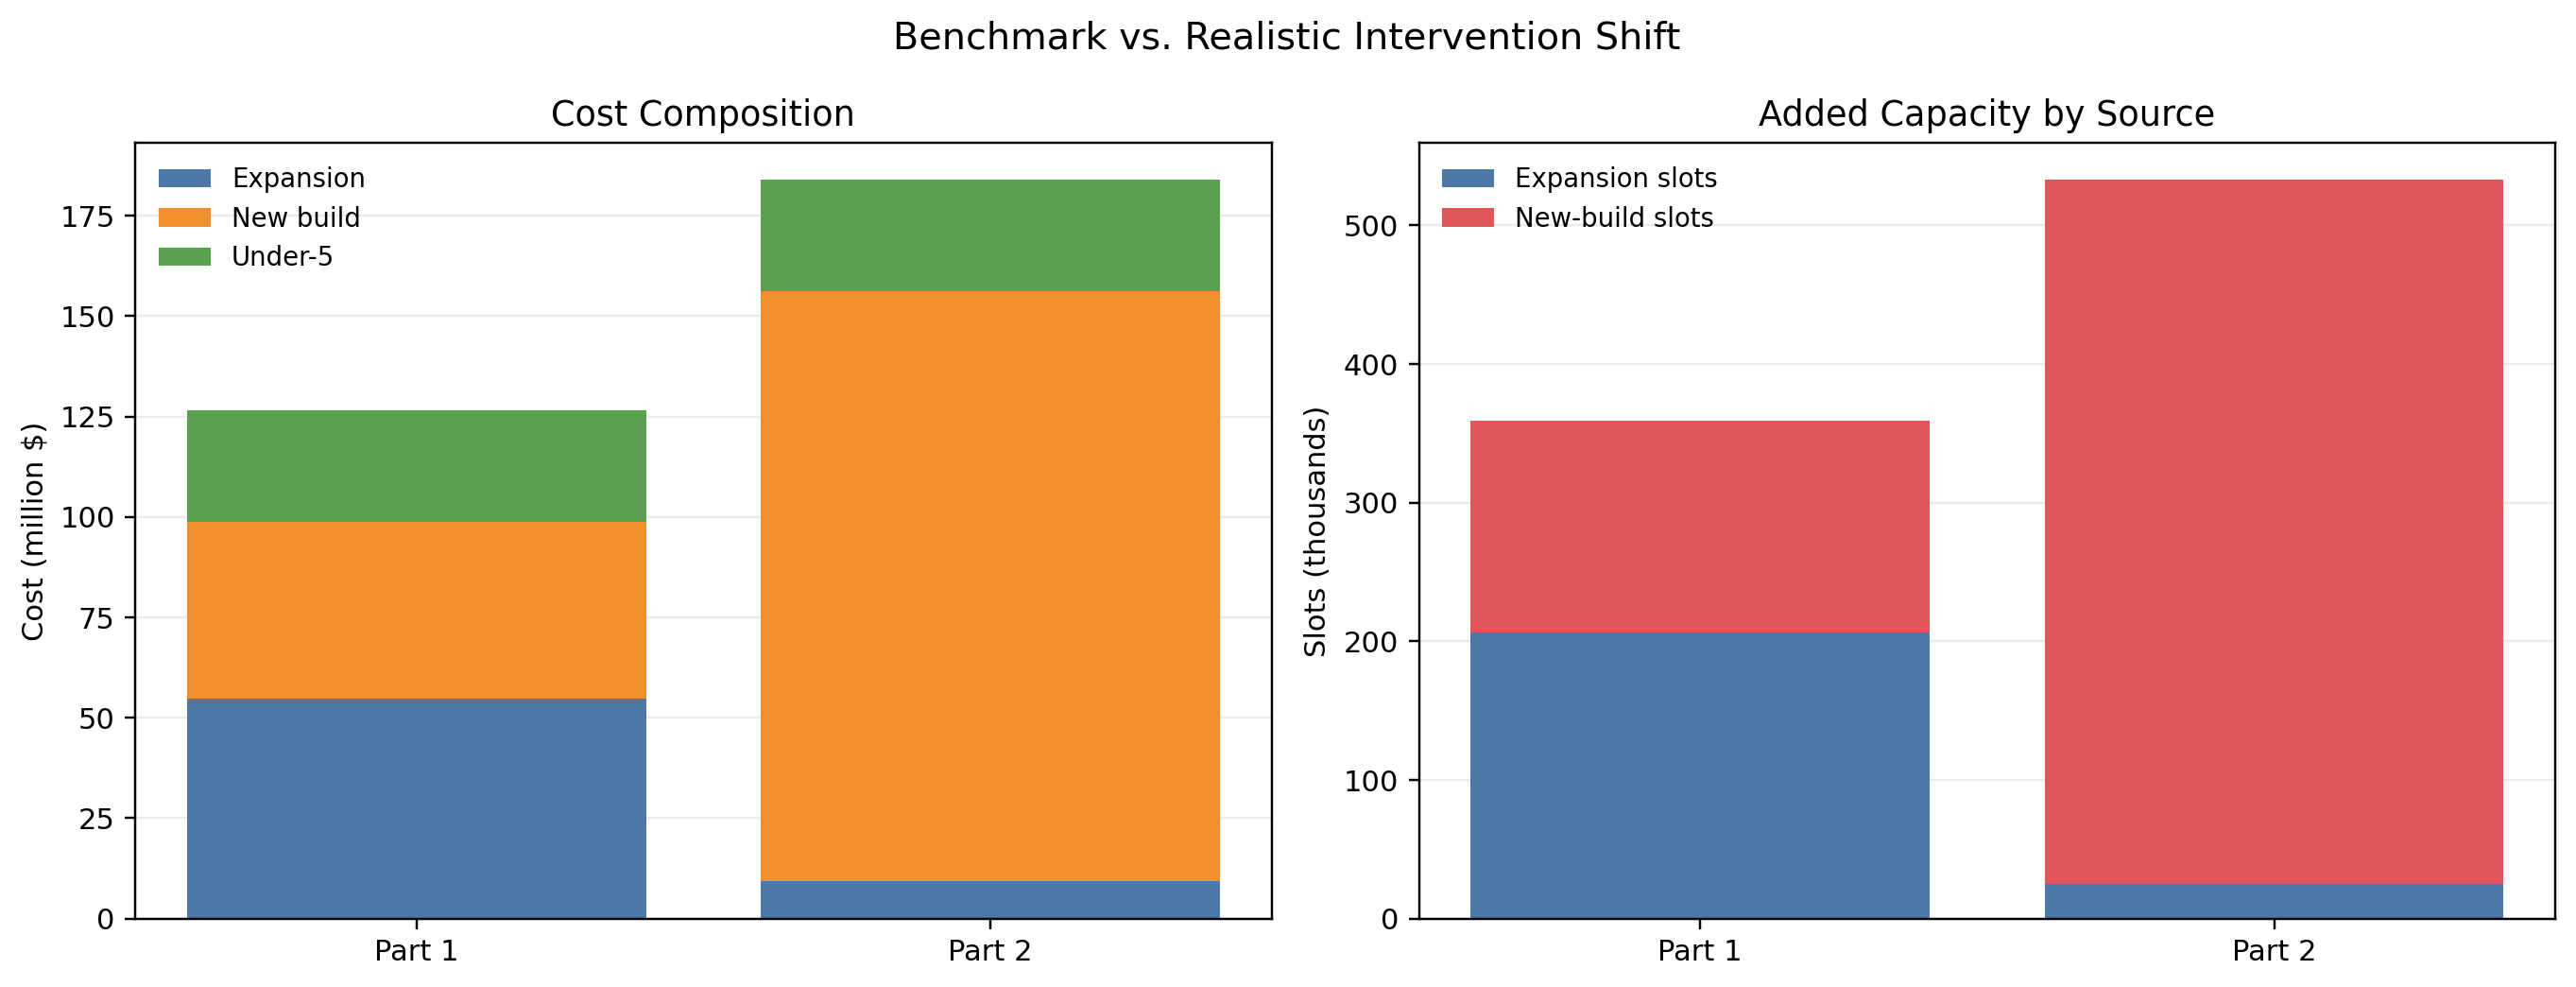
\includegraphics[width=0.94\textwidth]{part_comparison_overview.png}
\caption{Cost and capacity composition shift from Part 1 to Part 2}
\label{fig:comparison}
\end{figure}

\begin{figure}[H]
\centering
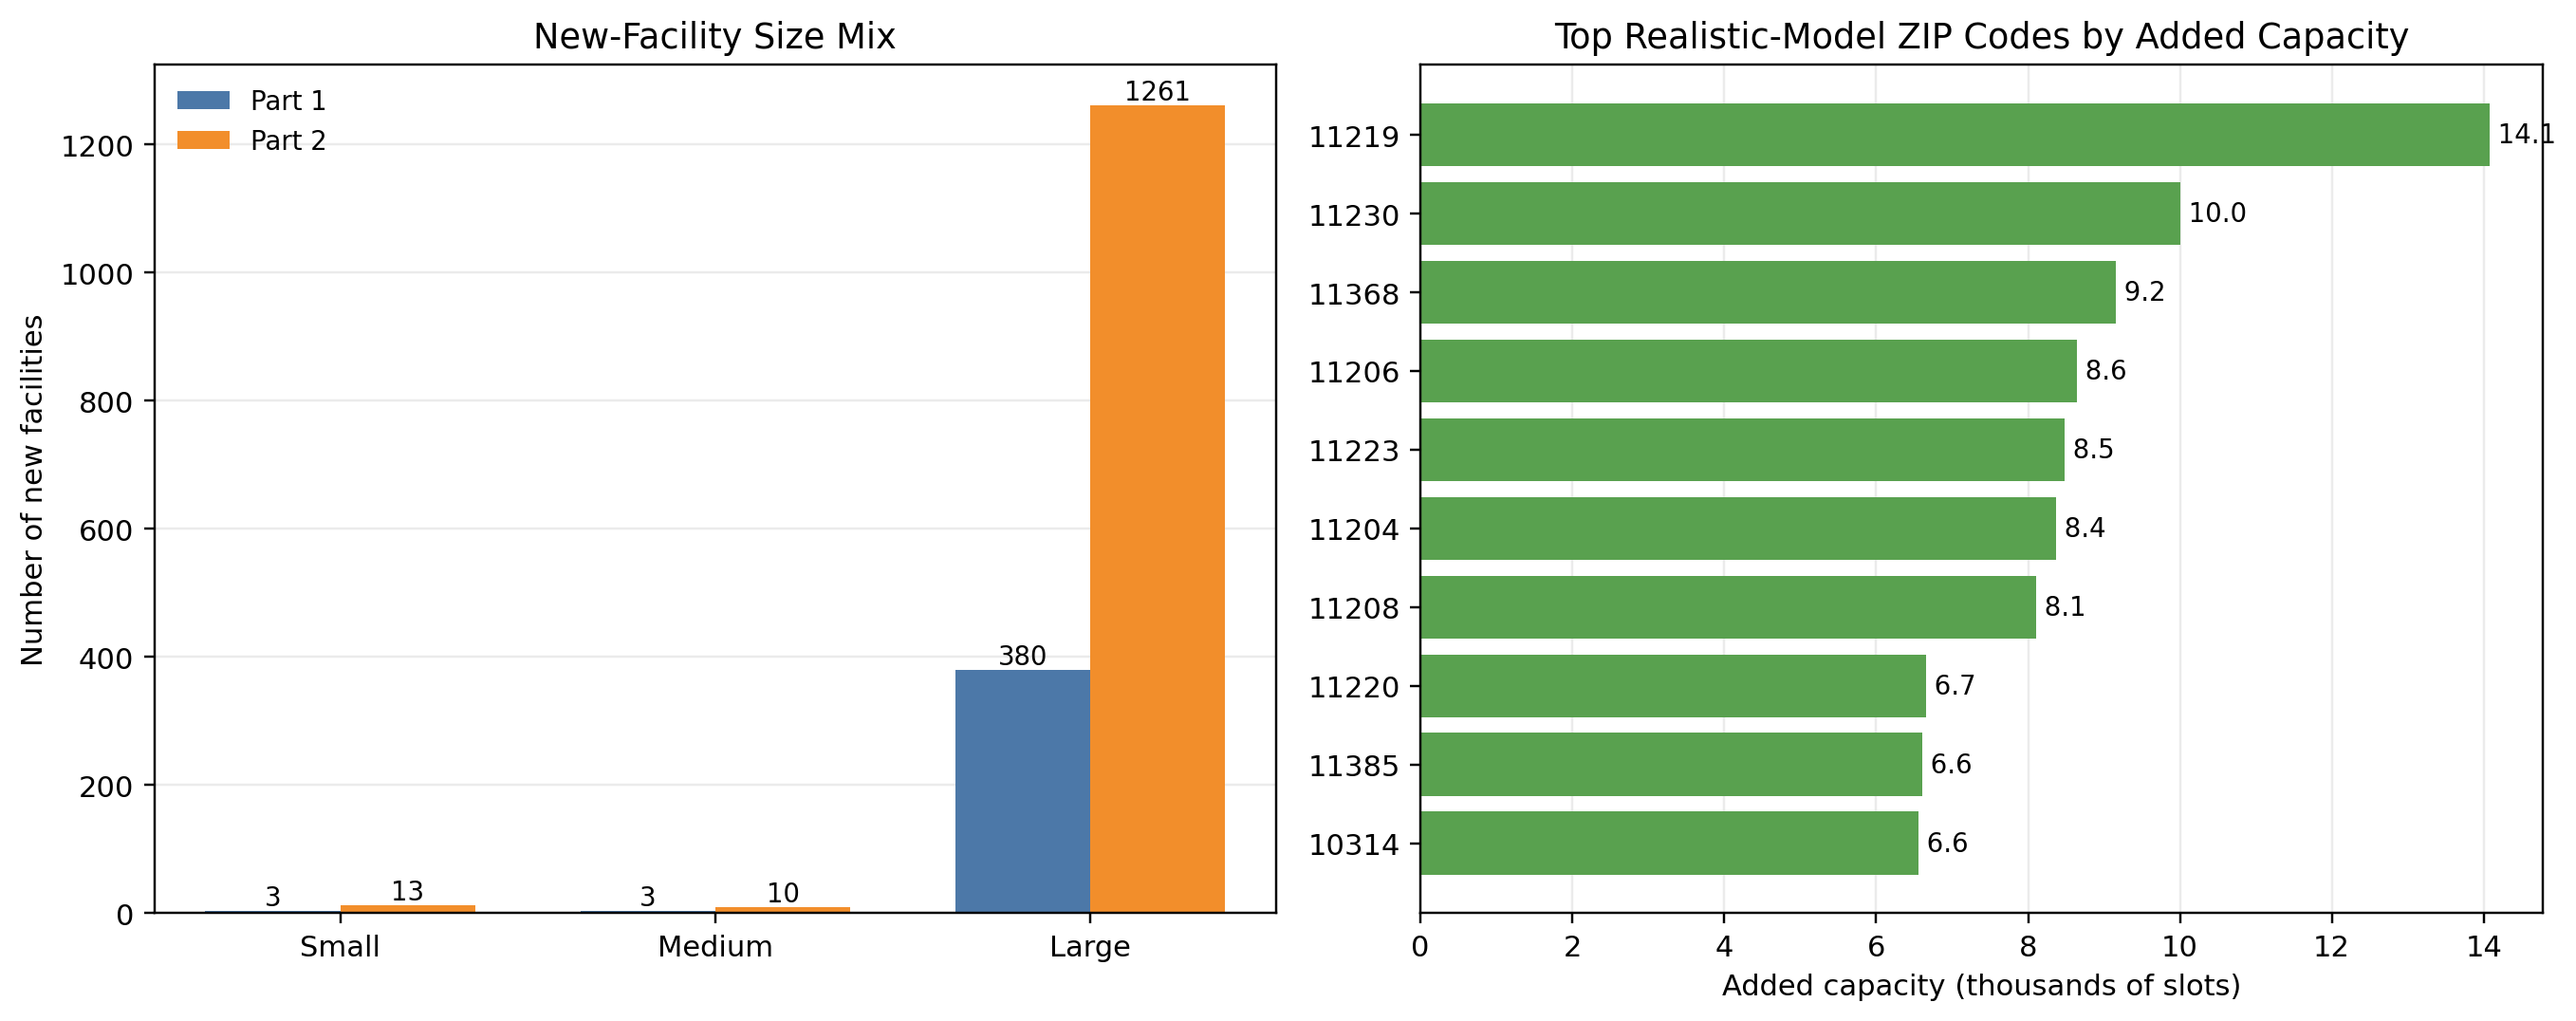
\includegraphics[width=0.94\textwidth]{realistic_mix_and_zipcodes.png}
\caption{Part 2 size mix and top zip codes by added capacity}
\label{fig:realistic-mix}
\end{figure}

Two patterns stand out. First, the realistic solution is dominated by large new facilities: \(1{,}261\) of the \(1{,}284\) selected new builds are large. Second, the under-\(5\) service requirement binds everywhere in the final realistic solution: all \(311\) zip codes have zero under-\(5\) slack, while only \(130\) have zero total-capacity slack. The model therefore creates visible total-capacity oversupply in order to meet the under-\(5\) requirement with the available build menu.

\section{Conclusions}

The seven-stage notebook pipeline supports a clear benchmark-to-realistic comparison. Under the implemented benchmark model, NYC can eliminate coded childcare deserts for \(\$126.67\) million. Under the implemented realistic model, the cost rises to \(\$183.96\) million because the city loses flexible siting and can expand incumbent facilities only modestly.

The key policy insight is that realistic implementation constraints change the structure of optimal intervention. Once expansion limits become binding and candidate-site spacing restrictions reduce the feasible siting set, the solution shifts away from incumbent expansion toward many more large new facilities. Across both parts, the under-\(5\) requirement remains the dominant planning driver, often forcing excess total capacity to satisfy age-specific targets.

\begin{thebibliography}{9}

\bibitem{assignment}
IEOR E4004.
\emph{Project I: Eliminating Child Care Deserts in New York City through Optimization}.
Columbia University, Spring 2026.

\bibitem{factsheet}
IEOR E4004.
\emph{Project I: Eliminating Child Care Deserts in New York City through Optimization --- Fact Sheet}.
Columbia University, Spring 2026.

\bibitem{americanprogress}
Center for American Progress.
\emph{Child Care Deserts in the United States}.
\url{https://www.americanprogress.org/series/child-care-deserts/}.

\end{thebibliography}

\end{document}
